\documentclass{beamer}
\usepackage{amsmath,amssymb,amsthm,tikz,color,wrapfig}
\usetheme{metropolis}
\setbeamertemplate{footline}[default]

\definecolor{azure}{rgb}{0.4, 0.2, 1.0}
\definecolor{cinnamon}{rgb}{0.82, 0.41, 0.12}
\definecolor{bur}{rgb}{0.6, 0.0, 0.0}

\title{Computing Galois groups of Fano problems}
\author{Thomas Yahl\\  \texttt{thomasjyahl@tamu.edu}\\ \vspace{-.1cm} \\ \texttt{arXiv:}\\ \vspace{-.1cm} \\ Texas A\&M University}
\date{June 2022}


\theoremstyle{definition}
\newtheorem{thm}{Theorem}

\setbeamersize{text margin left=8mm,text margin right=8mm} 

%%%%%%%%%%%%
%%Commands%%
%%%%%%%%%%%%
\newcommand{\new}[1]{{\color{black!15!blue}#1}}
\newcommand{\blue}[1]{{\color{black!15!blue}\underline{#1}}}
\newcommand{\orange}[1]{{\color{black!15!cinnamon}\underline{#1}}}


%%%%%%%%%%%%%%%%%
%%Rough Outline%%
%%%%%%%%%%%%%%%%%
%Computing Galois groups of Fano problems
%
%1. 27 lines (1 slide + picture)
%      mention "remakable configuration of lines"
%      Fano problems are generalizations of this
%   
%2. Fano problems (1 slide w/ example)
%      definition
%      dimension/degree (DM)
%      finite Fano problems
%      (1,6,(2,2,3)) example
%   
%3. Galois groups (2 slide + picture/gif?)
%      incidence variety
%      Galois group is monodromy group
%      path lifting (w/ picture)
%   
%4. Known results (1 slide)
%      Jordan/Harris for 27 lines
%      Hoshimoto & Kadets
%      remaining problems are alternating or symmetric
%      explore and prove with numerics
%
%5. Monodromy via homotopy continuation (3 slides, "would like to turn into proof")
%      necessary homotopy continuation slide (w/ picture)
%      small discriminant loop output for 27 lines and (1,6,(2,2,3))
%      computations, this is evidence we want proof
%
%6. Harris' method (1 slide + picture)
%      (1,n,(2n-3)) have symmetric Galois groups
%      Harris' method of proof (w/ picture)
%      this can be done computationally
%
%7. Certification (maybe 3 slides? picture? emphasize hard certification)
%      Smale's alpha theory
%      interval arithmetic
%      Shub's simple double roots
%
%8. Computations
%      constructing systems with unique simple double roots
%      certifying them w/ alpha theory/interval arithmetic + Shub
%      timings
%
%9. Moving forward
%      more computations
%      proving the result for all Fano problems
%

\begin{document}

%title frame
\begin{frame}
\titlepage

\texttt{arXiv:}
\end{frame}



%27 lines
%%mention "remakable configuration of lines"
%%Fano problems are generalizations of this
\begin{frame}
\frametitle{The problem of lines on a cubic surface}
\hspace{-.8cm}
\begin{minipage}{.55\textwidth}
\begin{enumerate}
\item[$\bullet$] Cayley and Salmon showed there are 27 distinct lines that lie on a smooth cubic surface.

\item[$\bullet$] Schl\"{a}fli determined these lines lie in a ``remarkable configuration'' 

\item[$\bullet$] A \blue{Fano problem} is the problem of enumerating linear spaces of a fixed dimension on a variety.
\end{enumerate}
\end{minipage}
%
\begin{minipage}{.02\textwidth}
~
\end{minipage}
%
\begin{minipage}{.4\textwidth}
%27 lines picture
\begin{center}
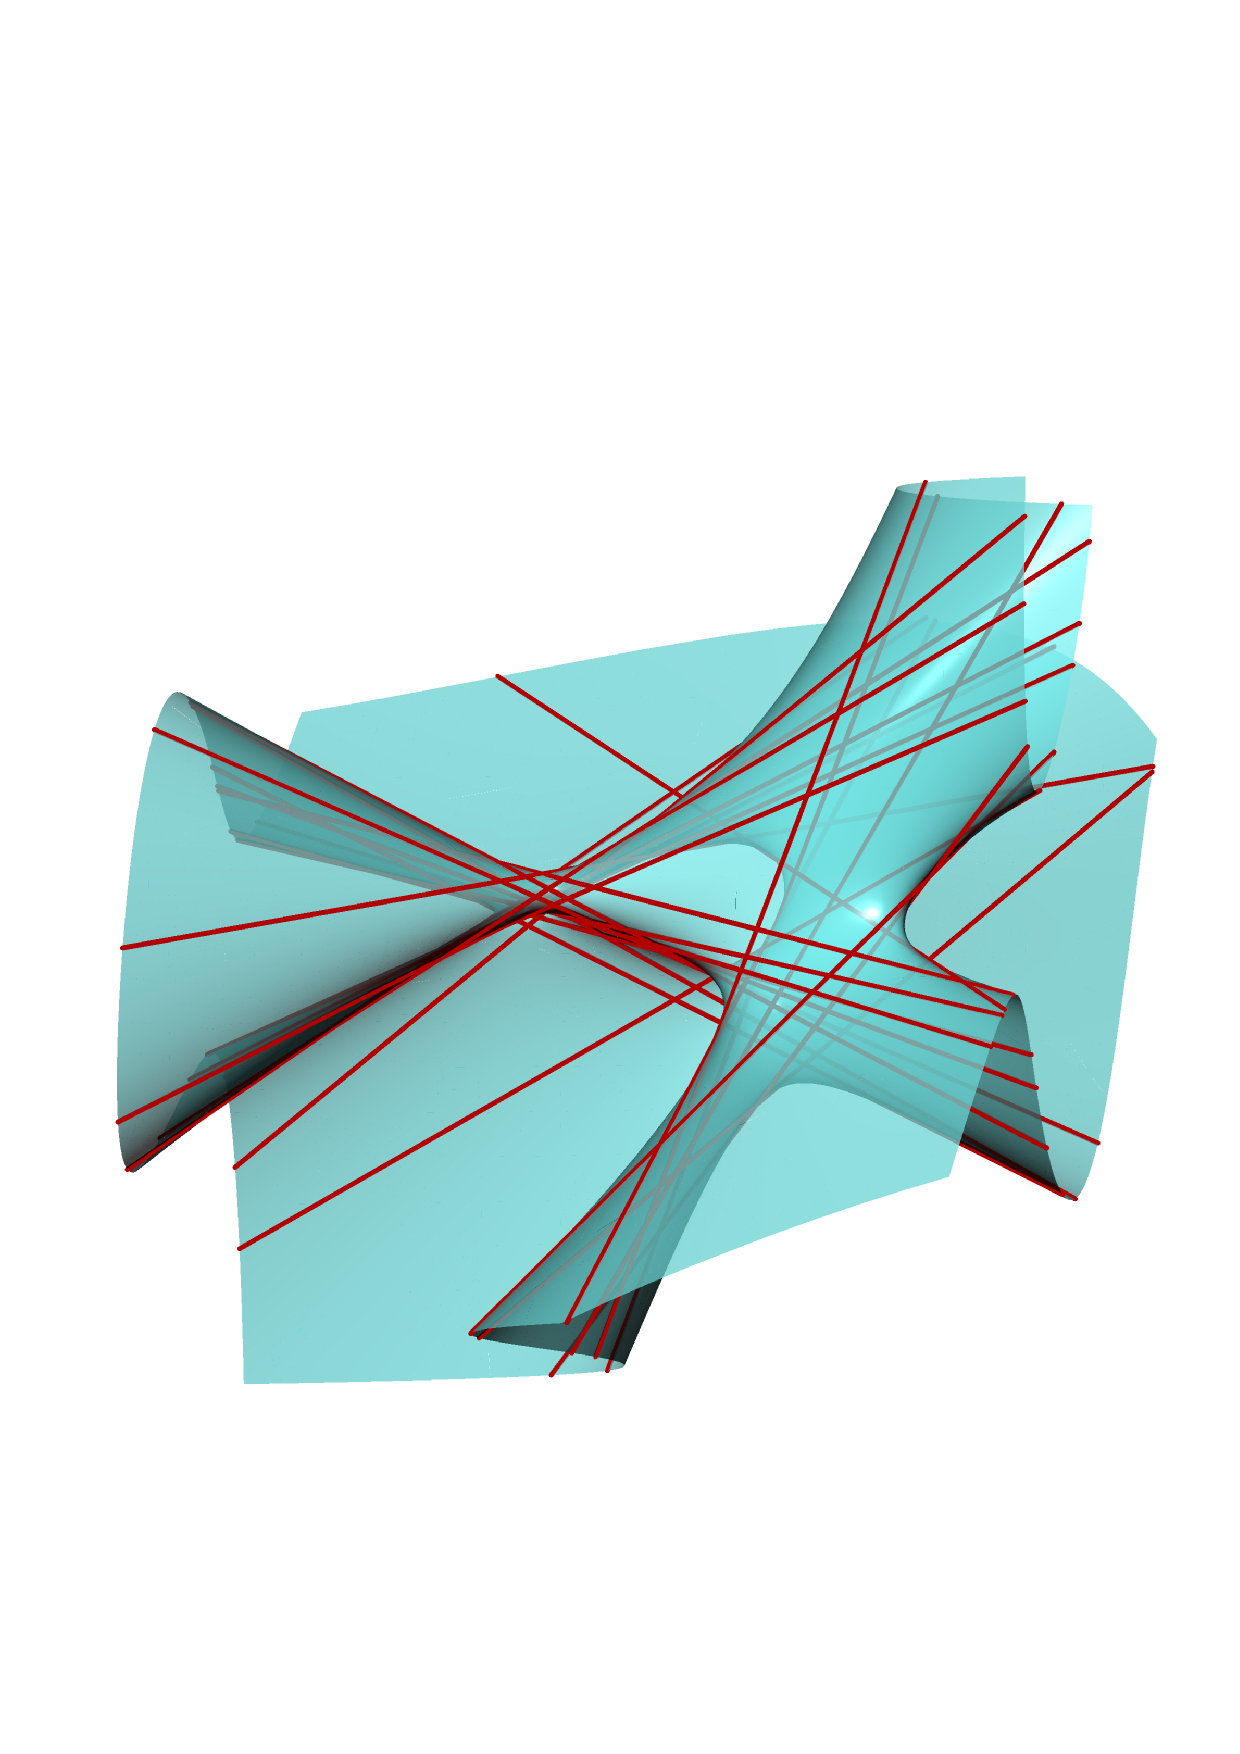
\includegraphics[scale=.32]{figures/27lines.pdf}
\end{center}
\end{minipage}


\end{frame}



%Fano problems
%%definition
%%dimension/degree (DM)
%%finite Fano problems
\begin{frame}
\frametitle{Fano problems}
\begin{enumerate}
\item[$\bullet$] For fixed degrees $d_\bullet = (d_1,\dotsc,d_s)$ choose homogeneous polynomials in $n+1$ variables, $F = (f_1,\dotsc,f_s)$.

\item[$\bullet$] Enumerate the $r$-planes that lie on the zero set $X_F = V(F)\subseteq\mathbb{P}^n$.
\end{enumerate}

When there are finitely many such $r$-planes for general polynomials $F = (f_1,\dotsc,f_s)$, this is a \blue{Fano problem} determined by $(r,n,d_\bullet)$.

\begin{enumerate}
\pause

\item[$\bullet$] The \blue{Fano scheme} $V_r(X_F)$ is the set of $r$-planes on $X_F$ as a subvariety of the Grassmanian $\mathbb{G}(r,\mathbb{P}^n)$.

\pause

\item[$\bullet$] The combinatorial data $(r,n,d_\bullet)$ determines a Fano problem when $n-s-2r\ge 0$ and

\vspace{-.8cm}

\begin{align*}
(r+1)(n-r) - \sum_{i=1}^s \left(\begin{smallmatrix}d_i + r\\r\end{smallmatrix}\right)=0.
\end{align*}
\end{enumerate}

\end{frame}


%
\begin{frame}
\frametitle{Examples}
Debarre and Manivel explicitly determined the number of solutions to the Fano problem determined by the data $(r,n,d_\bullet)$ by intersection theoretic means. Write this number as $\deg(r,n,d_\bullet)$.

We list all Fano problems with less than 1000 solutions below.

\begin{table}[htb]
  \label{Small Fano}
  \def\arraystretch{1.1}
  \begin{tabular}{||c|c|c|c|c||}
    \hline
    $r$ & $n$ & $d_\bullet$ & $\deg(r,n,d_\bullet)$ & Galois group\\
    \hline\hline
    1 & 4 & $(2,2)$ & 16 & $D_5$\\
    \hline
    1 & 3 & $(3)$ & 27 & $E_6$\\
    \hline
    2 & 6 & $(2,2)$ & 64 & $D_7$\\
    \hline
    3 & 8 & $(2,2)$ & 256 & $D_9$\\
    \hline
    1 & 7 & $(2,2,2,2)$ & 512 & \new{$S_{512}$}\\
    \hline
    1 & 6 & $(2,2,3)$ & 720  & \new{$S_{720}$}\\
    \hline
  \end{tabular}
\end{table}
\end{frame}



%Galois groups
%%incidence variety
%%Galois group is monodromy group
%%path lifting
\begin{frame}
\frametitle{Incidence correspondence}
Write $\mathbb{C}^{(r,n,d_\bullet)}$ for the parameter space of homogeneous forms $F = (f_1,\dotsc,f_s)$ in $n+1$ variables of degrees $d_\bullet = (d_1,\dotsc,d_s)$.

Fix $(r,n,d_\bullet)$. There is an incidence correspondence

\vspace{-.3cm}

\begin{center}
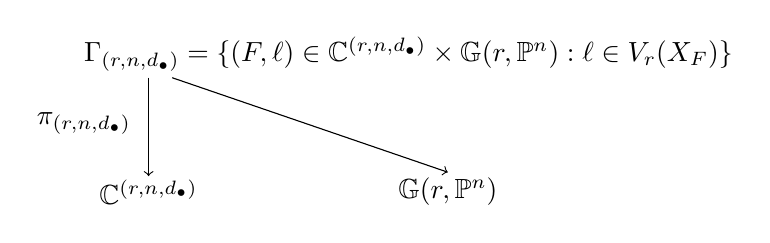
\begin{tikzpicture}
\node at (0,0) {$\Gamma_{(r,n,d_\bullet)} = \{(F,\ell)\in \mathbb{C}^{(r,n,d_\bullet)}\times\mathbb{G}(r,\mathbb{P}^n):\ell\in V_r(X_F)\}$};
\node at (-3.3,-1.75) {$\mathbb{C}^{(r,n,d_\bullet)}$};
\draw[->] (-3.3,-.3)--(-3.3,-1.55) node[left] at (-3.4,-.875) {$\pi_{(r,n,d_\bullet)}$};
\draw[->] (-3,-.3)--(.5,-1.5) node at (.5,-1.75) {$\mathbb{G}(r,\mathbb{P}^n)$};
\end{tikzpicture}
\end{center}

\vspace{-.45cm}

\begin{enumerate}
\item[$\bullet$] $\Gamma_{(r,n,d_\bullet)}$ is irreducible.

\item[$\bullet$] $\deg \pi_{(r,n,d_\bullet)} = \deg(r,n,d_\bullet)$ and the fiber over $F\in\mathbb{C}^{(r,n,d_\bullet)}$ is the set of $r$-planes $V_r(X_F)$.

\item[$\bullet$] $\pi_{(r,n,d_\bullet)}$ restricts to a covering space over a Zariski open set.
\end{enumerate}
\end{frame}



\begin{frame}
\frametitle{Galois groups of Fano problems}
\hspace{-.65cm}
\begin{minipage}{.73\textwidth}
\begin{enumerate}
\item[$\bullet$] The \blue{Galois group}, $\mathcal{G}_{(r,n,d_\bullet)}$, of the Fano problem determined by $(r,n,d_\bullet)$ is the monodromy group of $\pi_{(r,n,d_\bullet)}$.

\vspace{.1cm}

\item[$\bullet$] Jordan/Harris: $\mathcal{G}_{(1,3,(3))} = E_6$

\vspace{.1cm}

\item[$\bullet$] Harris: $\mathcal{G}_{(1,n,(2n-3))}$ is symmetric for $n\ge 4$

\vspace{.1cm}

\item[$\bullet$] Hashimoto/Kadets: $\mathcal{G}_{(r,2r+2,(2,2))} = D_{2r+3}$

\vspace{.1cm}

\item[$\bullet$] Hashimoto/Kadets: If $d_\bullet\ne(3),(2,2)$ then $\mathcal{G}_{(r,n,d_\bullet)}$ contains the alternating group
\end{enumerate}
\end{minipage}
%
\begin{minipage}{.25\textwidth}
\begin{center}
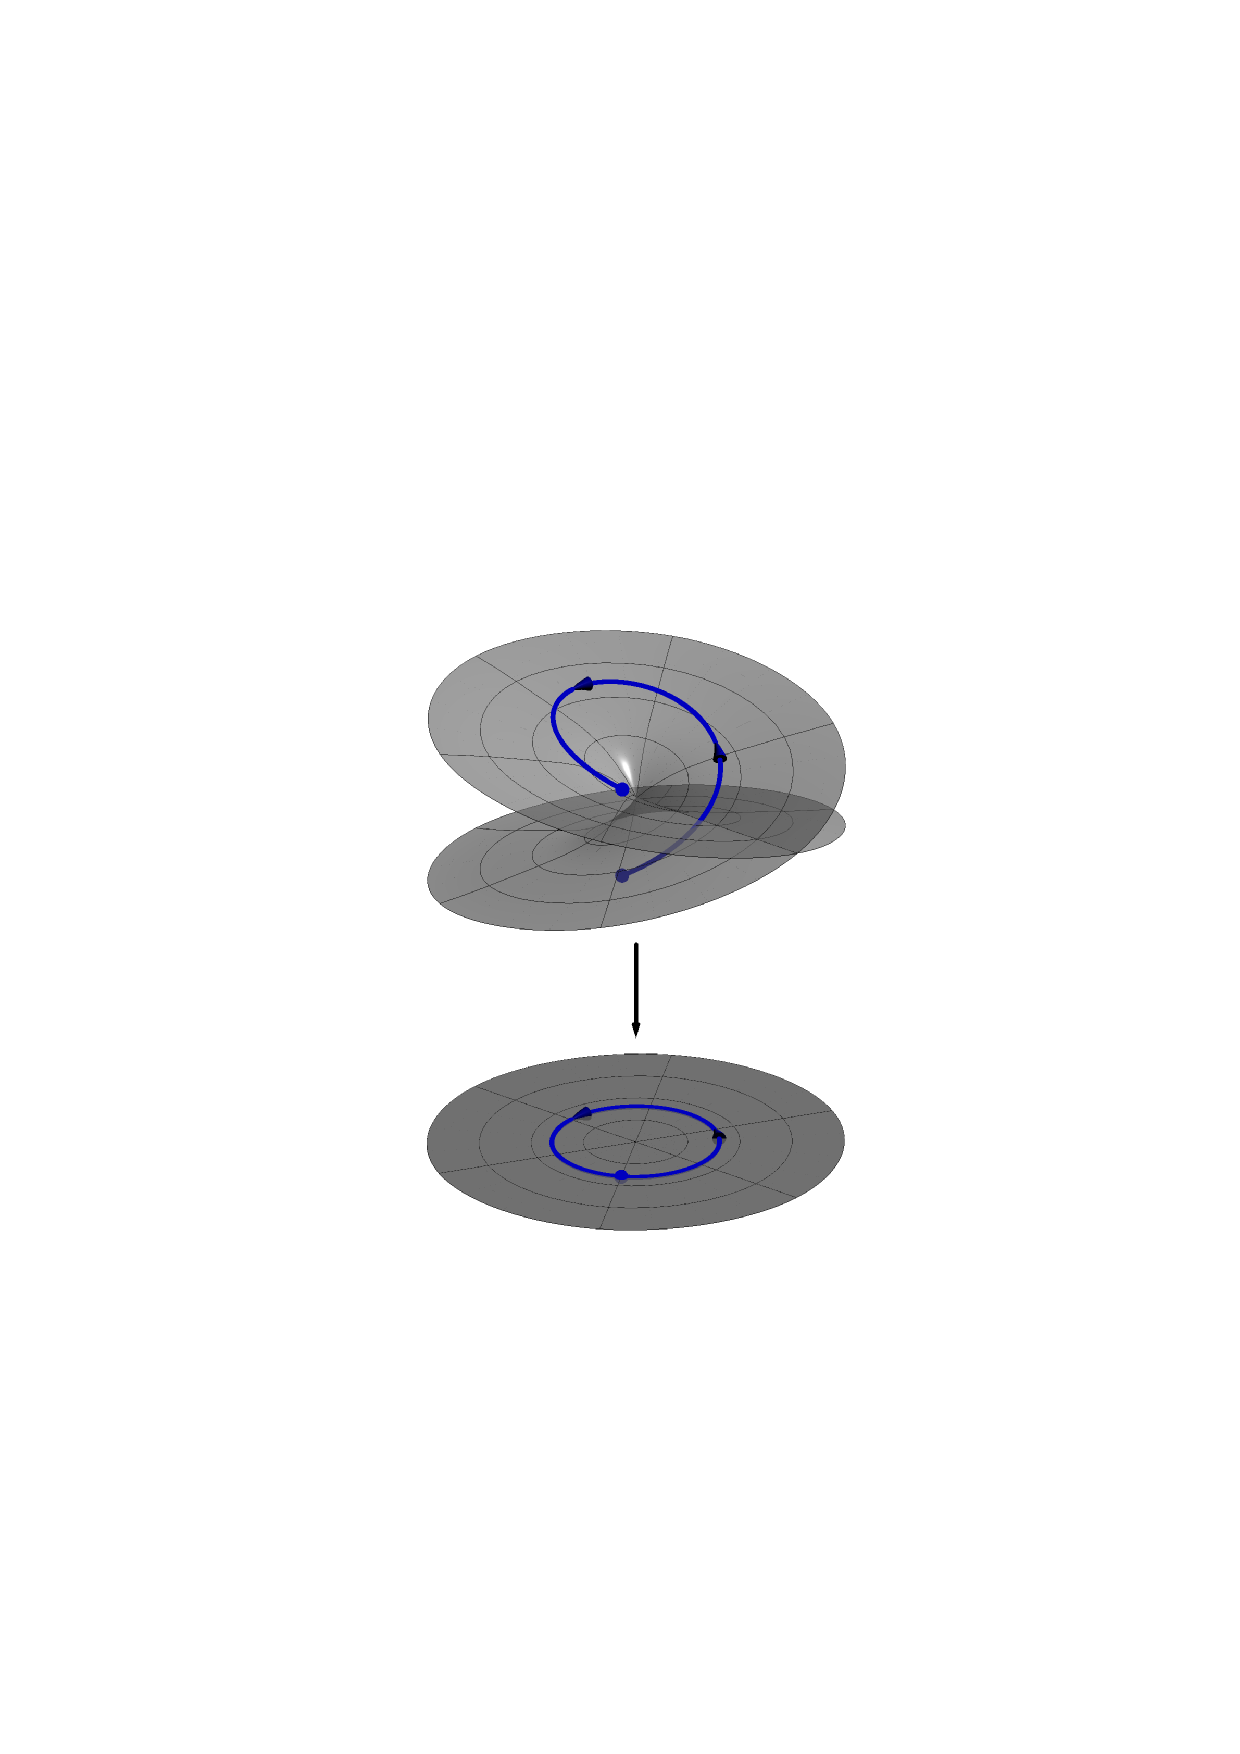
\includegraphics[scale=.5]{figures/monodromy.pdf}
\end{center}
\end{minipage}

\end{frame}


%Monodromy via homotopy continuation (2 slides, "would like to turn into proof")
%%necessary homotopy continuation slide (w/ picture)
%%small discriminant loop output for 27 lines and (1,6,(2,2,3))
%%computations, this is evidence we want proof
%\begin{frame}
%\frametitle{Numerical homotopy continuation}


%Numerical homotopy picture
%\begin{center}
%\begin{tikzpicture}
%\draw[thick,<->] (-2.75,0)--(2.75,0) node [right] at (2.75,0) {$t$};
%\draw[dashed] (-2,-.75)--(-2,1.75) node [below] at (-2,-.75) {$\mathcal{F}$};
%\draw[dashed] (2,-.75)--(2,1.75) node [below] at (2,-.75) {$\mathcal{G}$};

%\draw[blue,fill=blue] (2,-.3) circle (.05cm);
%\draw[blue,fill=blue] (-2,.3) circle (.05cm);
%\draw[blue,thick] (2,-.3)..controls(.9,-.5)..(.2,.6)..controls(-.1,1)..(-.65,.8);
%\draw[blue,thick] (-.85,.7)..controls(-1,.65)..(-2,.3);

%\draw[black!30!green,fill=black!30!green] (2,.15) circle (.05cm);
%\draw[black!30!green,fill=black!30!green] (-2,1.5) circle (.05cm);
%\draw[black!30!green,thick] (2,.15)..controls(1.5,.3)..(.8,-.1);
%\draw[black!30!green,thick] (.6,-.2)..controls(.3,-.3)..(-.3,.35)..controls(-1,1)..(-2,1.5);

%\draw[black!15!red,fill=black!15!red] (2,1.4) circle (.05cm);
%\draw[black!15!red,thick] (2,1.4)..controls(1.2,1)..(.4,1.2)..controls(-.5,1.4)..(-1,1.1);
%\draw[black!15!red,thick] (-1.2,.9)..controls(-1.3,.8)..(-1.45,.6);
%\draw[black!15!red,thick,->] (-1.6,.35)..controls(-1.75,.1)..(-1.85,-.6);
%\end{tikzpicture}
%\end{center}


%\end{frame}


%\begin{frame}
%\frametitle{Computations}

%\end{frame}



%Harris' method
%%Harris' method of proof
\begin{frame}
\frametitle{Harris' method of proof}
%\textbf{\underline{Goal:}} use numerics \underline{prove} remaining Galois groups contain a simple transposition and are therefore symmetric. 

%\vspace{.2cm}

\begin{lemma}[Harris]

\vspace{.05cm}

Let $\pi:Y\mapsto Z$ be a smooth map of degree $k$ between irreducible varieties. If there exists a point $p\in Z$ such that the fiber $\pi^{-1}(p)$ consists of exactly $k-2$ simple points and one double point then the monodromy group of $\pi$ contains a simple transposition.
\end{lemma}

\vspace{.2cm}

We have a smooth map $\pi_{(r,n,d_\bullet)}:\Gamma_{(r,n,d_\bullet)}\to\mathbb{C}^{(r,n,d_\bullet)}$ of degree $\deg(r,n,d_\bullet)$ between irreducible varieties.
\begin{enumerate}
\item[$\bullet$] Heuristically choose $F\in\mathbb{C}^{(r,n,d_\bullet)}$ so that $V_r(X_F)$ consists of $\deg(r,n,d_\bullet)-2$ simple points and one double point.

\item[$\bullet$] Solve a system $\overline{F}$ describing $V_r(X_F)$ in local coordinates.

\item[$\bullet$] Verify claims with exact computation and numerical certification.
\end{enumerate}
\end{frame}





\begin{frame}
\frametitle{Choose $F\in\mathbb{C}^{(r,n,d_\bullet)}$, write $\overline{F}$, and solve}
Choose local coordinates on $\mathbb{G}(r,\mathbb{P}^n)$ and for $\omega\in\mathbb{G}(r,\mathbb{P}^n)$ use local coordinates $\omega^\ast$ to parameterize $\omega$.
\vspace{-.1cm}
\begin{enumerate}
\item[$\bullet$] Write $\overline{F}$ as the system sending local coordinates of $\omega\in\mathbb{G}(r,\mathbb{P}^n)$ to the coefficients of $F|_\omega$ in local coordinates on $\omega$.

\item[$\bullet$] Choose $\ell\in\mathbb{G}(r,\mathbb{P}^n)$ and a nonzero vector $v\in\mathbb{C}^{(r+1)(n-r)}$.

\item[$\bullet$] Randomly select $F\in\mathbb{C}^{(r,n,d_\bullet)}$ satisfying the linear conditions $\overline{F}(\ell^\ast)=0$ and $D\overline{F}(\ell^\ast)v=0$.

\item[$\bullet$] Use your favorite solver to enumerate the solutions of $\overline{F}$.
\end{enumerate}

\textbf{\underline{Note:}} If $\ell$ and $v$ have rational coordinates, $F$ can be chosen to have rational coordinates as well.
\end{frame}



%IMAGE??
\begin{frame}
\frametitle{Simple double roots and numerical certification}
A \blue{simple double root} of a system $G$ is a root $x$ satisfying $\ker DG(x) = \langle v \rangle$ and $D^2G(x)(v,v)\not\in \text{im}\,DG(x)$. 
\vspace{-.2cm}
\begin{enumerate}
\item[$\bullet$] By work of Shub, simple double roots are isolated solutions of multiplicity 2.

\item[$\bullet$] If $\ell$, $v$, and $F$ have rational coordinates, these conditions can be checked exactly.
\end{enumerate}

There are 2 methods of isolating the remaining solutions.
\vspace{-.2cm}
\begin{enumerate}
\item[$\bullet$] $\alpha$-theory 

\item[$\bullet$] Interval arithmetic
\end{enumerate}
\end{frame}



\begin{frame}
\frametitle{Smale's $\alpha$-theory}
Given a system $G:\mathbb{C}^m\to\mathbb{C}^m$ and $x\in\mathbb{C}^m$, there are associated quantities $\alpha(G,x)$, $\beta(G,x)$, and $\gamma(G,x)$. 

\begin{thm}[Smale et al.]
\vspace{-.1cm}
If $G$ is a system and $x$ is such that
\vspace{-.2cm}
\begin{align*}
\alpha(G,x) < \frac{13-3\sqrt{17}}{4},
\end{align*}
\vspace{-.85cm}

then $x$ converges (quadratically) under Newton's method to a solution $y$ of $G$. Further, $||x-y||\le 2\beta(G,x)$.
\end{thm}

\begin{enumerate}
\item[$\bullet$] When $G$ and $x$ are given by exact coordinates, this provides an exact isolating ball for the solution $y$. 

\item[$\bullet$] \texttt{alphaCertified} will check the inequality above and certify balls isolating solutions are disjoint, with exact arithmetic. 
\end{enumerate}
\end{frame}




\begin{frame}
\frametitle{Interval Arithmetic}
Given a system $G:\mathbb{C}^m\to\mathbb{C}^m$, $x\in\mathbb{C}^m$, and $Y\in\text{GL}_m(\mathbb{C})$, the Krawczyk operator $K_{x,Y}$ on the space of complex intervals generalizes the Newton operator.

\begin{thm}
\vspace{-.1cm}
If $G$ is a system, and $x$ is a point, and $I$ is a complex interval such that 
\vspace{-.3cm}
\begin{align*}
K_{x,Y}(I)\subseteq I,
\end{align*}
\vspace{-.85cm} 

then $I$ contains a zero of $G$.
\end{thm}

\begin{enumerate}
\item[$\bullet$] Certifies computations using floating point arithmetic.

\item[$\bullet$] \texttt{HomotopyContinuation.jl} will attempt to find a complex interval around an approximate solution to isolate solutions.
\end{enumerate}
\end{frame}





\begin{frame}
\frametitle{Results and timings}
\begin{thm}[Y.] 
\vspace{.01cm}
The Fano problems with $d_\bullet\ne (3),(2,2)$ and less than 40,000 solutions have full symmetric Galois group.
\end{thm}
\vspace{-.1cm}
\textbf{Timing:} (\texttt{NAG4M2},\texttt{alphaCertified},\texttt{HomotopyContinuation.jl})
\vspace{-.2cm}
\begin{table}[htb]
  \label{Small Fano}
  \def\arraystretch{.98}
  \begin{tabular}{||c|c|c|c|c|c||}
    \hline
    $r$ & $n$ & $d_\bullet$ & $\deg(r,n,d_\bullet)$ & $\texttt{M2}$ (h) & $\texttt{julia}$ (s)\\
    \hline\hline
    1 & 7 & $(2,2,2,2)$ & 512 & 2.66 & .61\\
    \hline
    1 & 6 & $(2,2,3)$ & 720  & 2.88 & .87\\
    \hline
    2 & 8 & $(2,2,2)$ & 1024 & 27.32 & 1.57\\
    \hline
    1 & 5 & (3,3) & 1053 & 2.69 & .32\\
    \hline
    1 & 5 & (2,4) & 1280 & 6.09 & .73\\
    \hline
    1 & 10 & (2,2,2,2,2,2) & 20480 & - & 15.44\\
    \hline
    1 & 9 & (2,2,2,2,3) & 27648 & - & 25.97\\
    \hline
    2 & 10 & (2,2,2,2) & 32768 & - & 36.67\\
    \hline
    1 & 8 & (2,2,3,3) & 37584 & - & 38.23\\
    \hline
  \end{tabular}
\end{table}
\end{frame}



%
\begin{frame}
\frametitle{Moving forward}
Data for these systems and code verifying the data is available at 
\vspace{-.25cm}
\begin{center}
\texttt{github.com/tjyahl/FanoGaloisGroups}
\end{center}
\vspace{-.25cm}
There is more to do!
\begin{enumerate}
\item[$\bullet$] Generate systems with a single simple double root for larger Fano problems (in progress).

\item[$\bullet$] Turn this into a proof for ALL Fano problems with $d_\bullet\ne(3),(2,2)$.

\item[$\bullet$] Explore using numerical certification for proving more about Galois groups.
\end{enumerate}
\end{frame}


\begin{frame}
\frametitle{References}
\begin{center}
\textbf{\underline{Thank you all for your time!}}
\end{center}
\end{frame}

\end{document}



